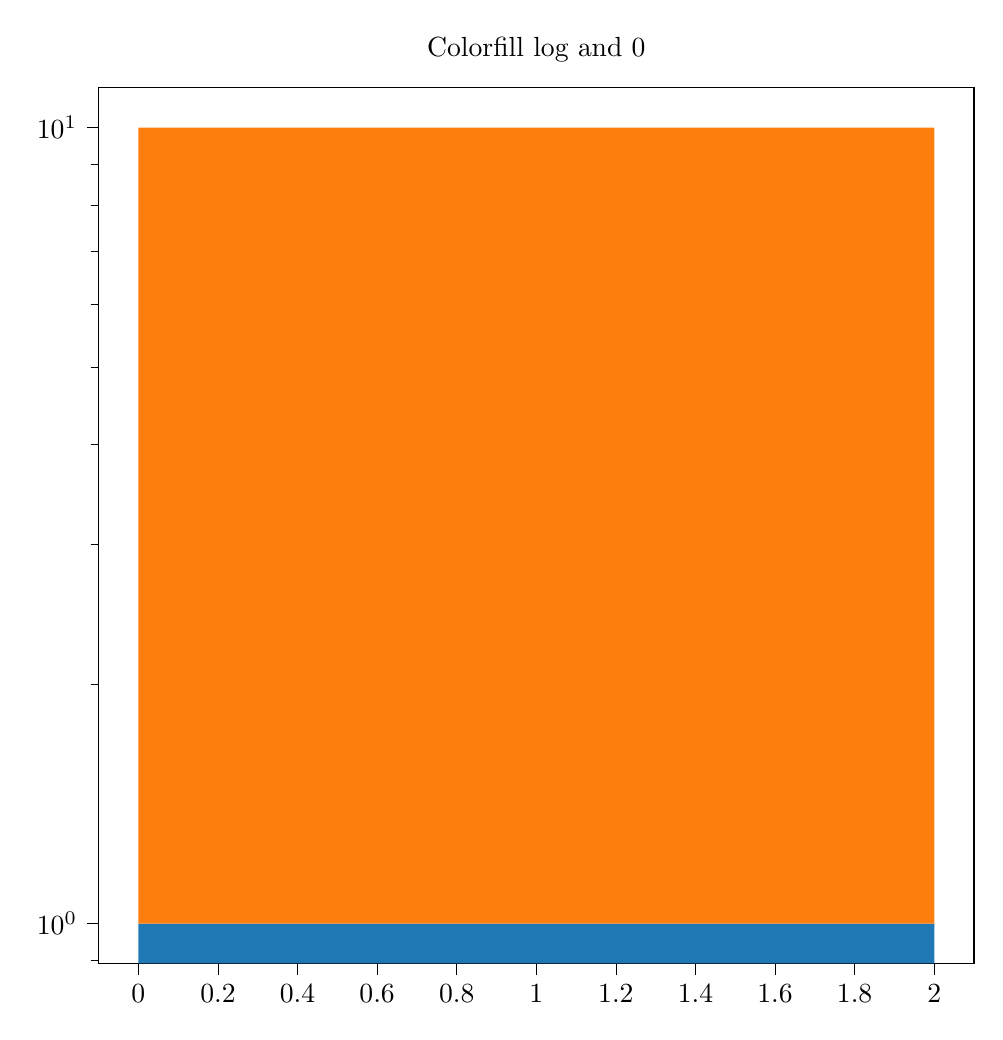
\begin{tikzpicture}

\definecolor{darkgray176}{RGB}{176,176,176}
\definecolor{darkorange25512714}{RGB}{255,127,14}
\definecolor{steelblue31119180}{RGB}{31,119,180}

\begin{axis}[
height=5in,
log basis y={10},
tick align=outside,
tick pos=left,
title={Colorfill log and 0},
width=5in,
x grid style={darkgray176},
xmin=-0.1, xmax=2.1,
xtick style={color=black},
y grid style={darkgray176},
ymin=0.89125094, ymax=11.220185,
ymode=log,
ytick style={color=black}
]
\path [fill=steelblue31119180]
(axis cs:0,1)
--(axis cs:0,0.89125094)
--(axis cs:1,0.89125094)
--(axis cs:2,0.89125094)
--(axis cs:2,1)
--(axis cs:2,1)
--(axis cs:1,1)
--(axis cs:0,1)
--cycle;

\path [fill=darkorange25512714]
(axis cs:0,10)
--(axis cs:0,1)
--(axis cs:1,1)
--(axis cs:2,1)
--(axis cs:2,10)
--(axis cs:2,10)
--(axis cs:1,10)
--(axis cs:0,10)
--cycle;

\end{axis}

\end{tikzpicture}
